\apendice{Documentación de usuario}

\section{Introducción}

En este apartado se detallan los requisitos necesarios para utilizar correctamente la aplicación web, así como el curso completo que debe seguir el usuario para usarla adecuadamente.

\section{Requisitos de usuarios}

Para el uso normal de la aplicación, el usuario solo necesita lo siguiente:

\begin{itemize}
    \item Un navegador web compatible como Firefox, Google Chrome, etc.
    \item Acceso a Internet.
    \item Acceder a la página web \texttt{https://tfg-traclus-2.onrender.com}.
    \item Tener un archivo de trayectorias válido, en formato Excel o CSV.
\end{itemize}

\section{Instalación}

En este caso, no debería ser necesaria la instalación de ningún software adicional, ya que la aplicación está diseñada para ejecutarse en un entorno web accesible a través del navegador. Solo es necesario contar con los requisitos mencionados anteriormente para usarla correctamente.

\section{Manual del usuario}

Esta aplicación fue creada con el objetivo de realizar pruebas en el algoritmo TRACLUS utilizando diferentes configuraciones de clústeres. El flujo de acciones en la aplicación está diseñado para ser sencillo y se divide en dos posibles caminos principales.

\subsection{Pantalla de inicio}

Nada más acceder a la aplicación, el usuario encontrará la página inicial. 

\begin{figure}[H]
    \centering
    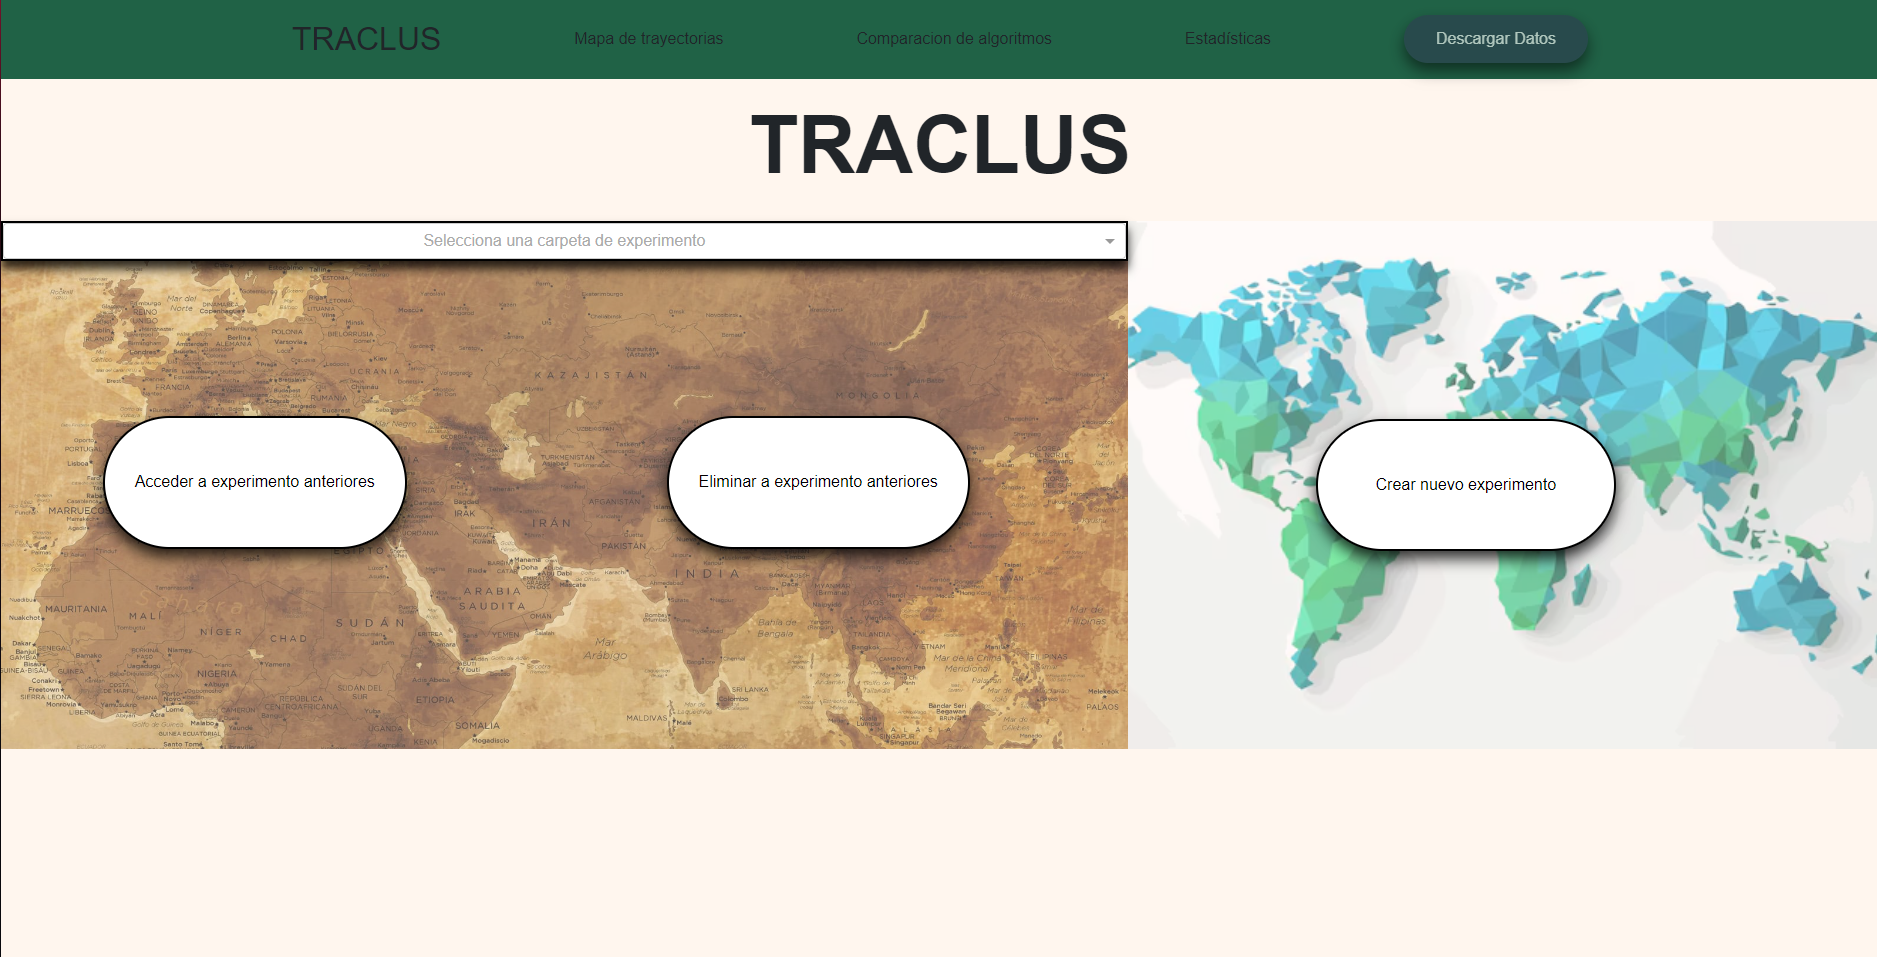
\includegraphics[width=0.9\textwidth]{img/webpage/main_page.png}
    \caption{Pantalla inicial de la aplicación}
\end{figure}

La barra de navegación en esta pantalla tiene todos los botones desactivados (indicados en color negro). Las opciones disponibles para el usuario dependen del estado de los experimentos existentes:

\begin{itemize}
    \item Si no existen experimentos, la única opción disponible será crear un nuevo experimento.
    \item Si ya hay experimentos creados, las opciones adicionales serán cargar o eliminar un experimento existente.
\end{itemize}

\subsection{Crear un nuevo experimento}

Si el usuario decide crear un nuevo experimento, será redirigido a una página donde podrá seleccionar los algoritmos y configurarlos. 

\begin{figure}[H]
    \centering
    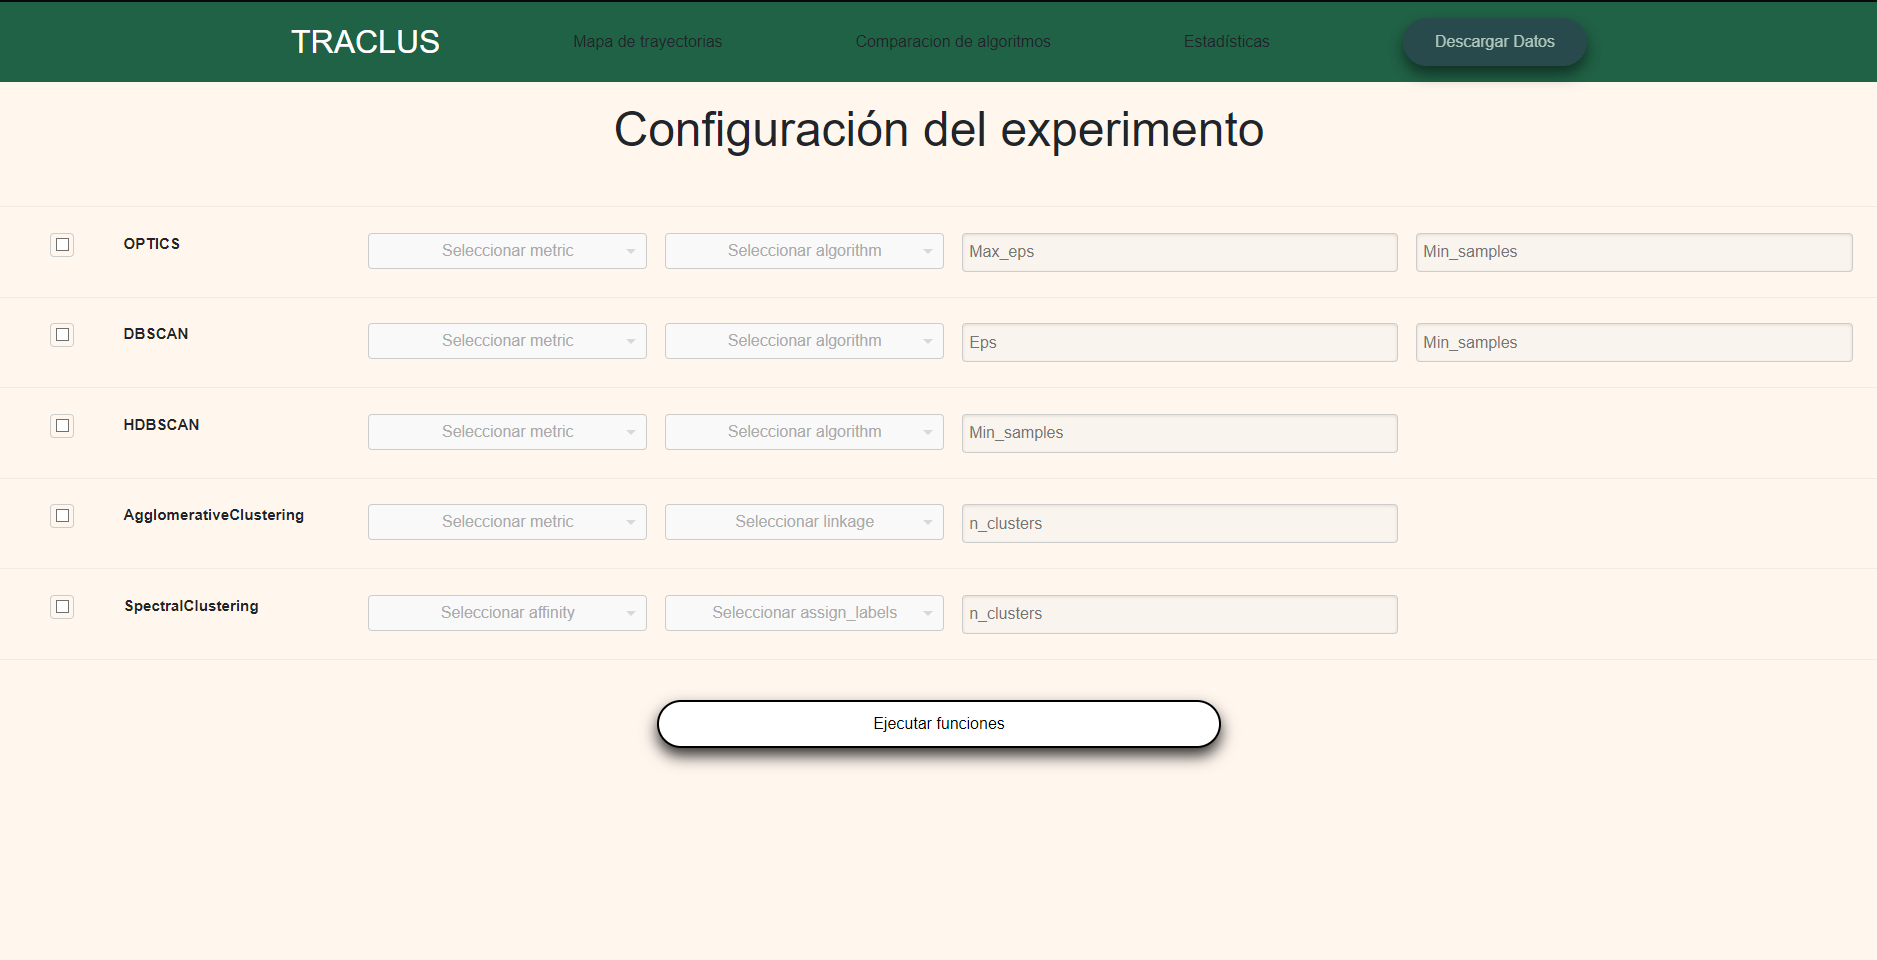
\includegraphics[width=0.9\textwidth]{img/webpage/experiment_page.png}
    \caption{Pantalla para la creación de un nuevo experimento}
\end{figure}

En esta página:

\begin{itemize}
    \item Solo estará habilitado el botón \texttt{Home} en la barra de navegación, permitiendo regresar a la pantalla inicial.
    \item El usuario debe seleccionar los algoritmos que desea utilizar y completar los parámetros requeridos para cada uno.
\end{itemize}

Al completar estos pasos, el botón inferior permitirá avanzar a la siguiente pantalla. Es importante destacar que este botón no estará activo hasta que se hayan configurado correctamente todos los algoritmos.

\begin{figure}[H]
    \centering
    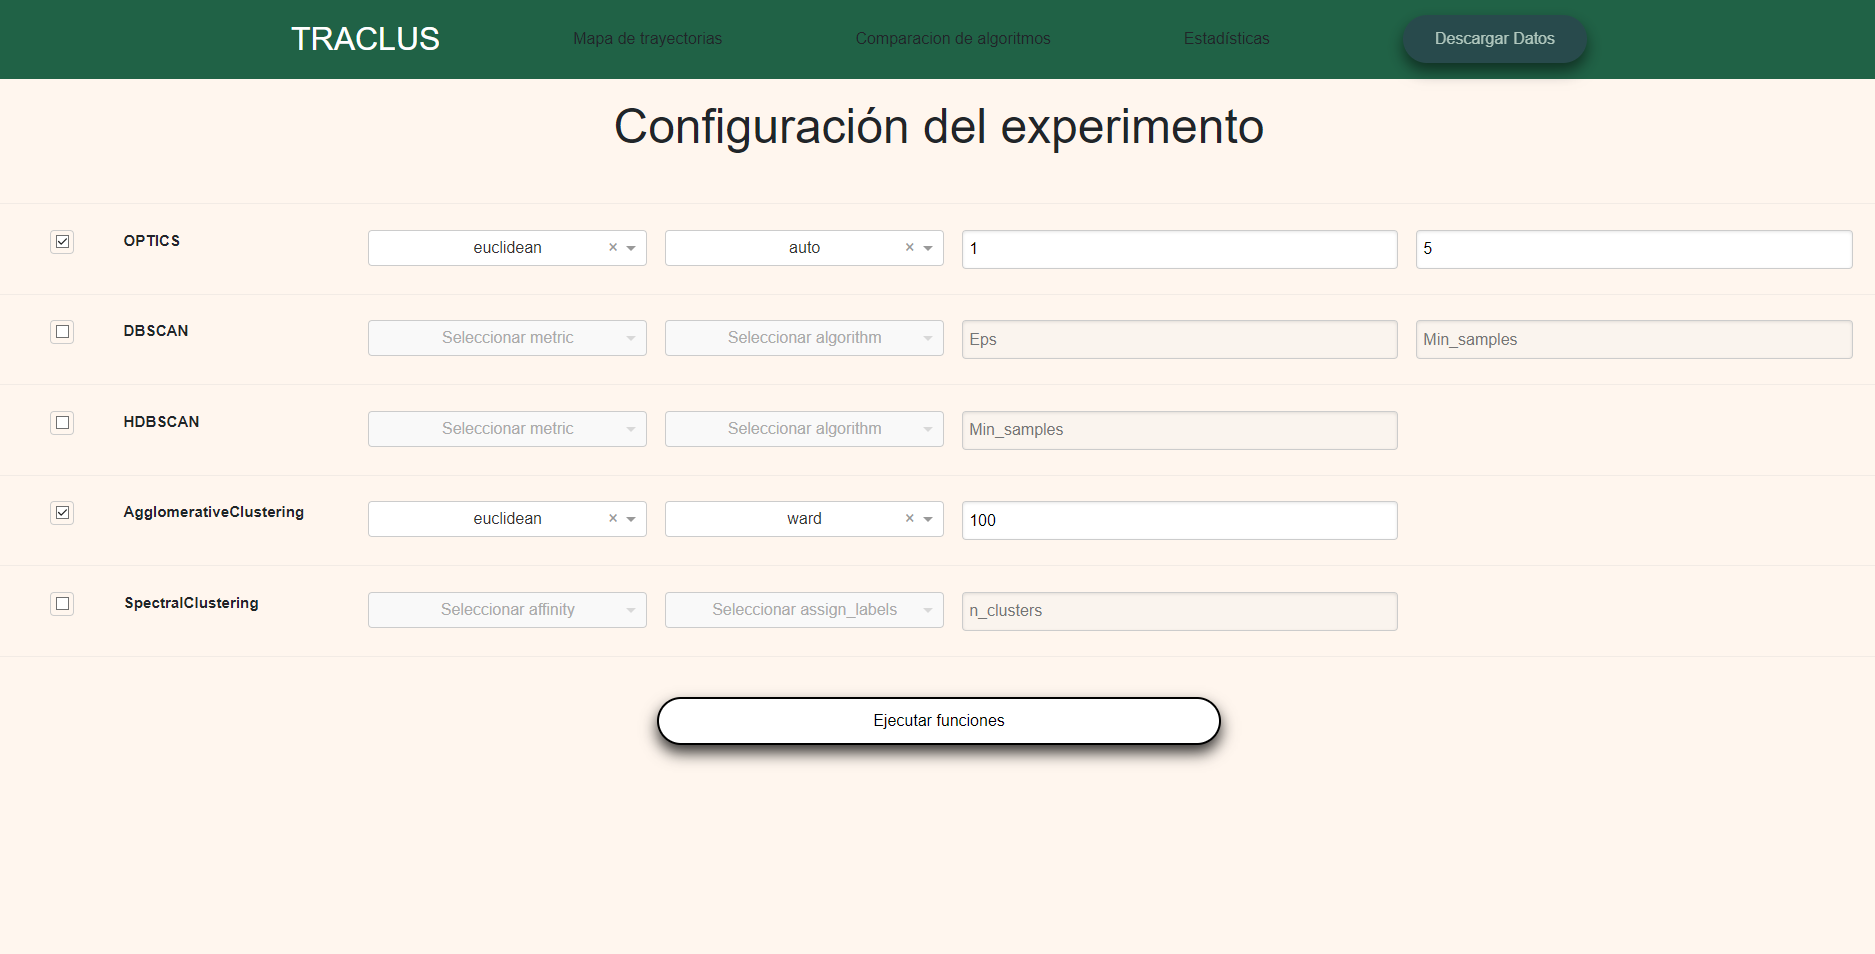
\includegraphics[width=0.9\textwidth]{img/webpage/experiment_page_complete.png}
    \caption{Pantalla para la creación de un nuevo experimento con datos}
\end{figure}

\subsection{Cargar datos}

En la pantalla de carga de datos, el usuario debe completar la información necesaria para iniciar el experimento.

\begin{figure}[H]
    \centering
    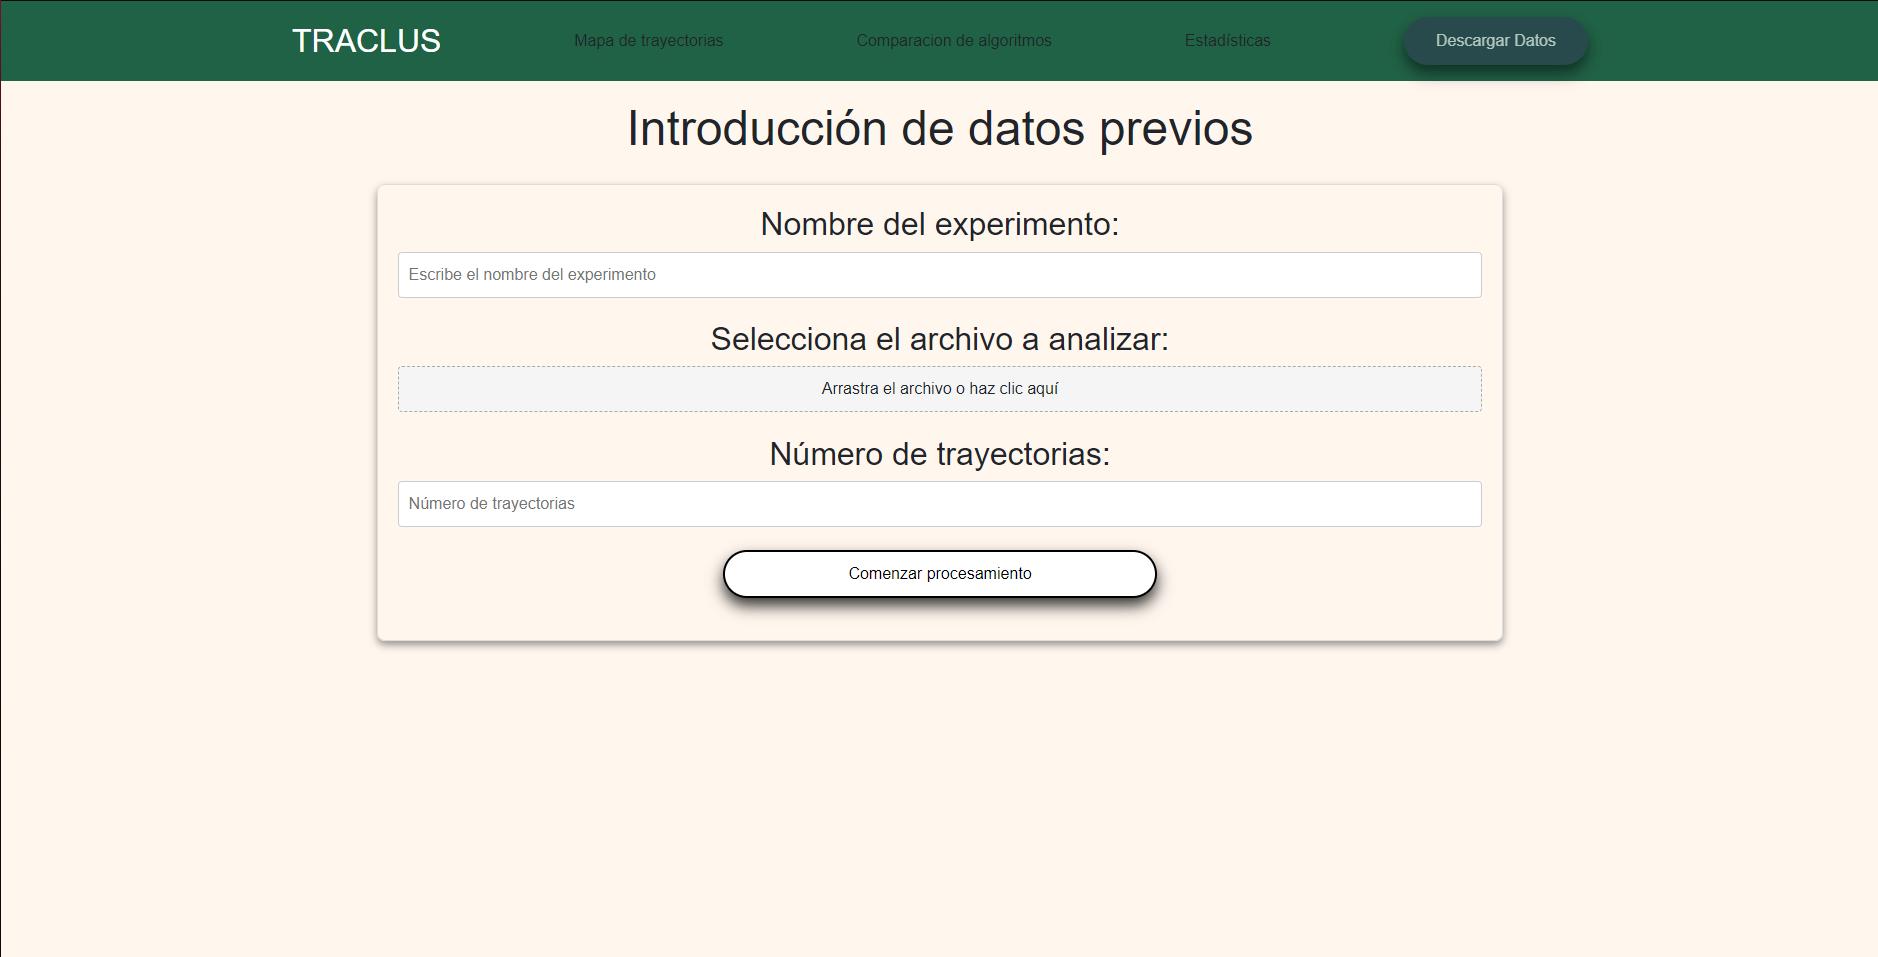
\includegraphics[width=0.9\textwidth]{img/webpage/load_page.png}
    \caption{Pantalla de carga de datos}
\end{figure}

En esta sección, se solicita:

\begin{itemize}
    \item Nombre del experimento.
    \item Archivo de datos en formato CSV o Excel.
    \item Número de datos a procesar del archivo seleccionado.
\end{itemize}

Al hacer clic en el botón de carga, el sistema procesará los datos. En caso de error, se mostrará un mensaje indicando la causa (datos incompatibles, parámetros incorrectos o fallos de conexión).

\begin{figure}[H]
    \centering
    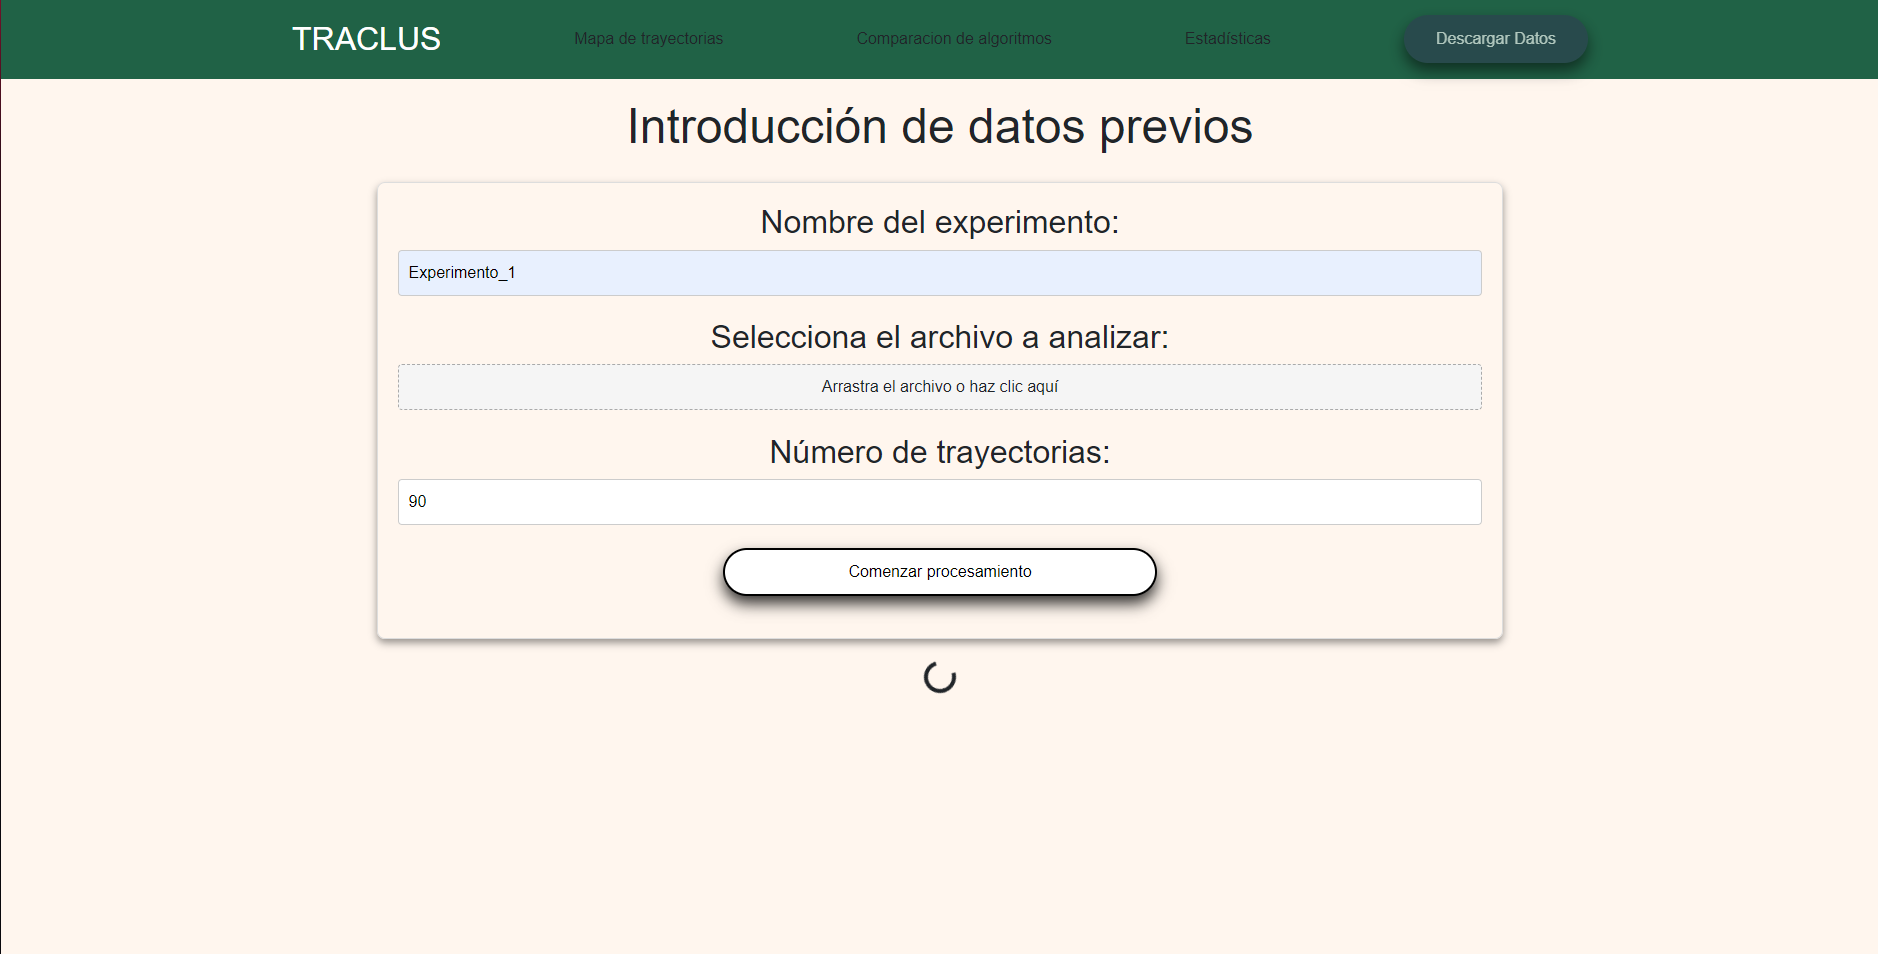
\includegraphics[width=0.9\textwidth]{img/webpage/load_page_loading.png}
    \caption{Pantalla de carga de datos cargando}
\end{figure}

\subsection{Visualización de resultados}

Si el procesamiento es exitoso, el usuario será redirigido a la página de mapas, donde se muestran los datos sin tratar en un mapa.

\begin{figure}[H]
    \centering
    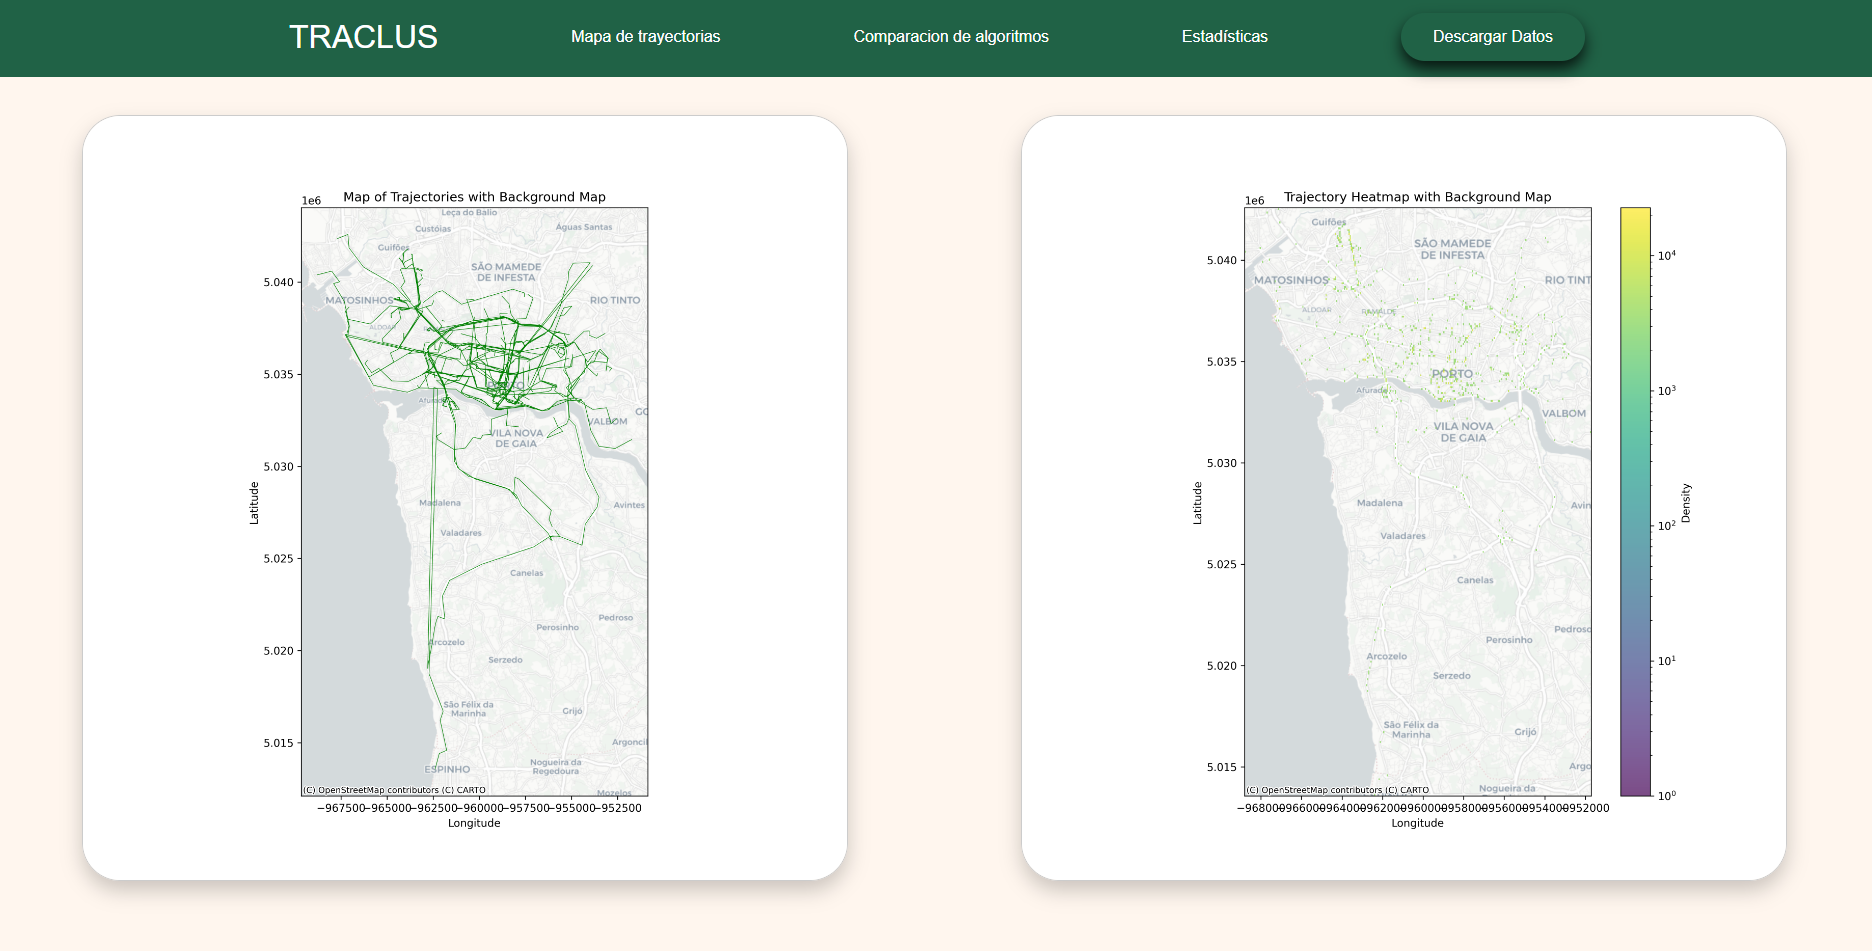
\includegraphics[width=0.9\textwidth]{img/webpage/Map_page.png}
    \caption{Pantalla de visualización de datos sin tratar}
\end{figure}

En esta etapa, la barra de navegación desbloqueará todos los botones:

\begin{itemize}
    \item \textbf{Comparación de algoritmos}: Muestra mapas con los resultados de los algoritmos.
    
\begin{figure}[H]
    \centering
    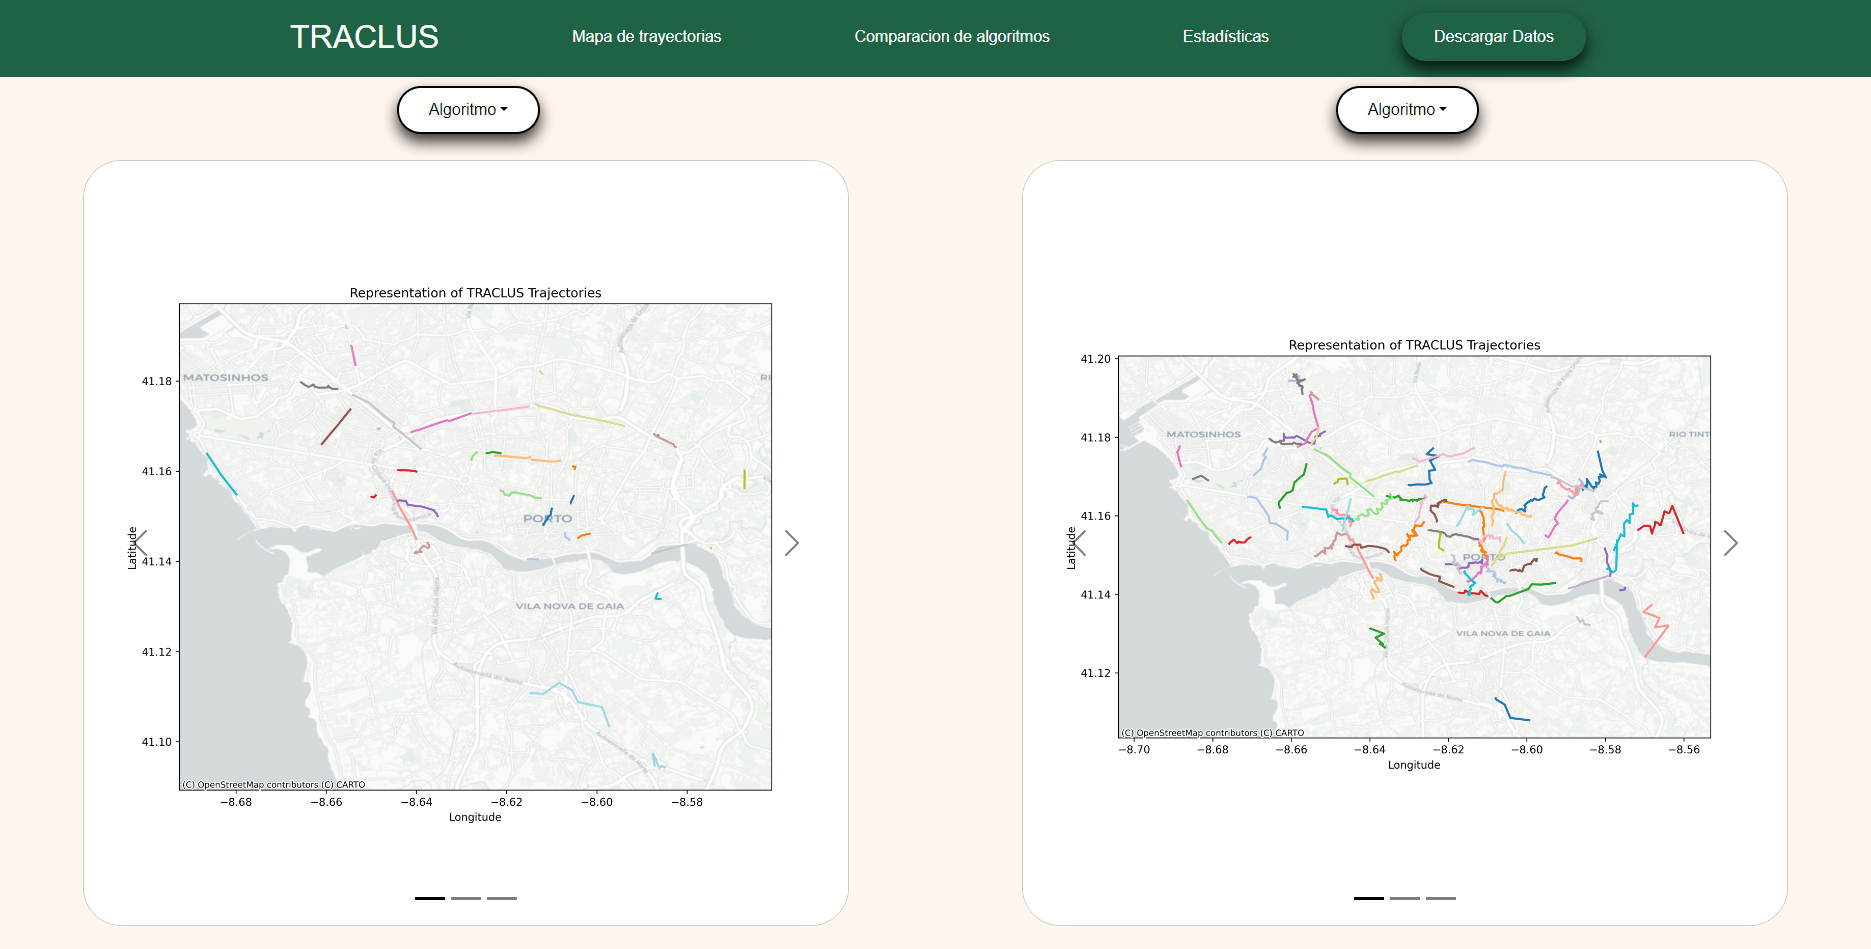
\includegraphics[width=0.9\textwidth]{img/webpage/TRACLUSMap_page.png}
    \caption{Pantalla de visualización de mapas con resultados representados}
\end{figure}
    
    \item \textbf{Estadísticas}: Proporciona una tabla con datos analíticos.
    
\begin{figure}[H]
    \centering
    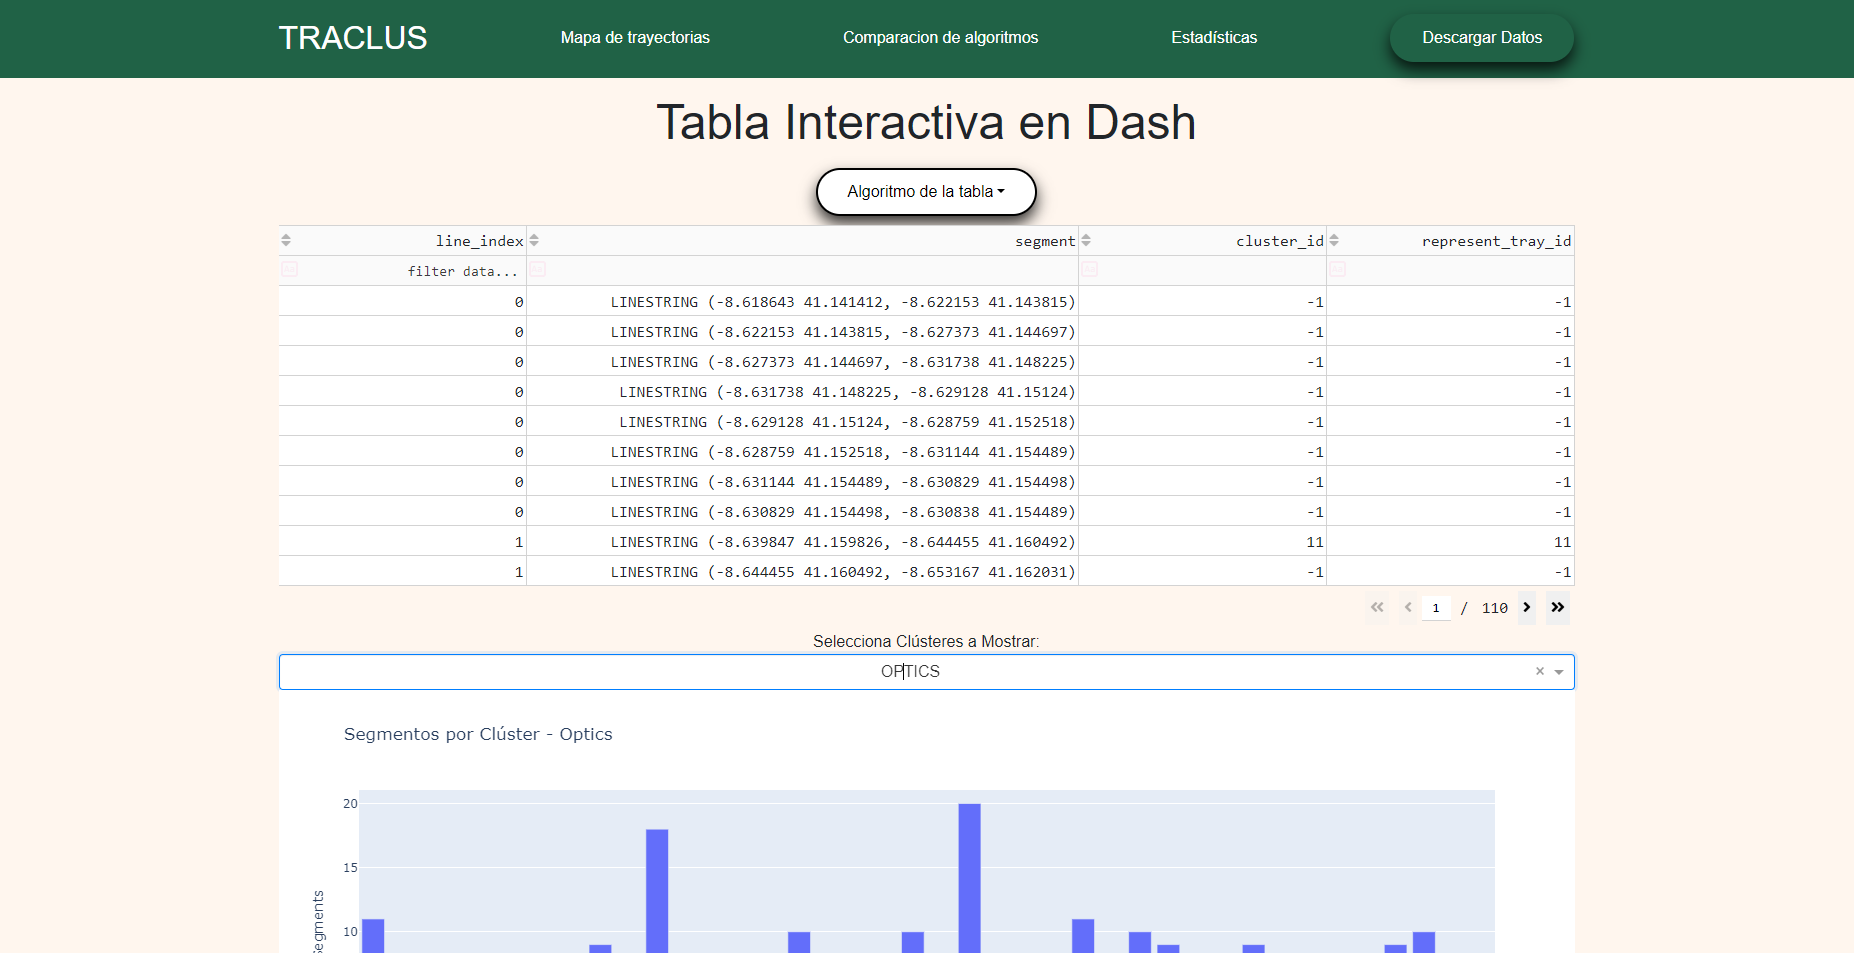
\includegraphics[width=0.9\textwidth]{img/webpage/estadistic_page.png}
    \caption{Pantalla de en bruto}
\end{figure}

    \item \textbf{Descargar}: Permite descargar un archivo ZIP con todos los datos procesados del experimento.
\end{itemize}

\subsection{Gestión de experimentos existentes}

Tras la creación de un experimento, el usuario puede volver a la pantalla inicial, donde tendrá nuevas opciones habilitadas:

\begin{itemize}
    \item \textbf{Cargar experimento existente}: Redirige directamente a la pantalla de mapas, con acceso a todas las funcionalidades.
    \item \textbf{Eliminar experimento}: Despliega un menú para confirmar la eliminación del experimento seleccionado.
\end{itemize}

\begin{figure}[H]
    \centering
    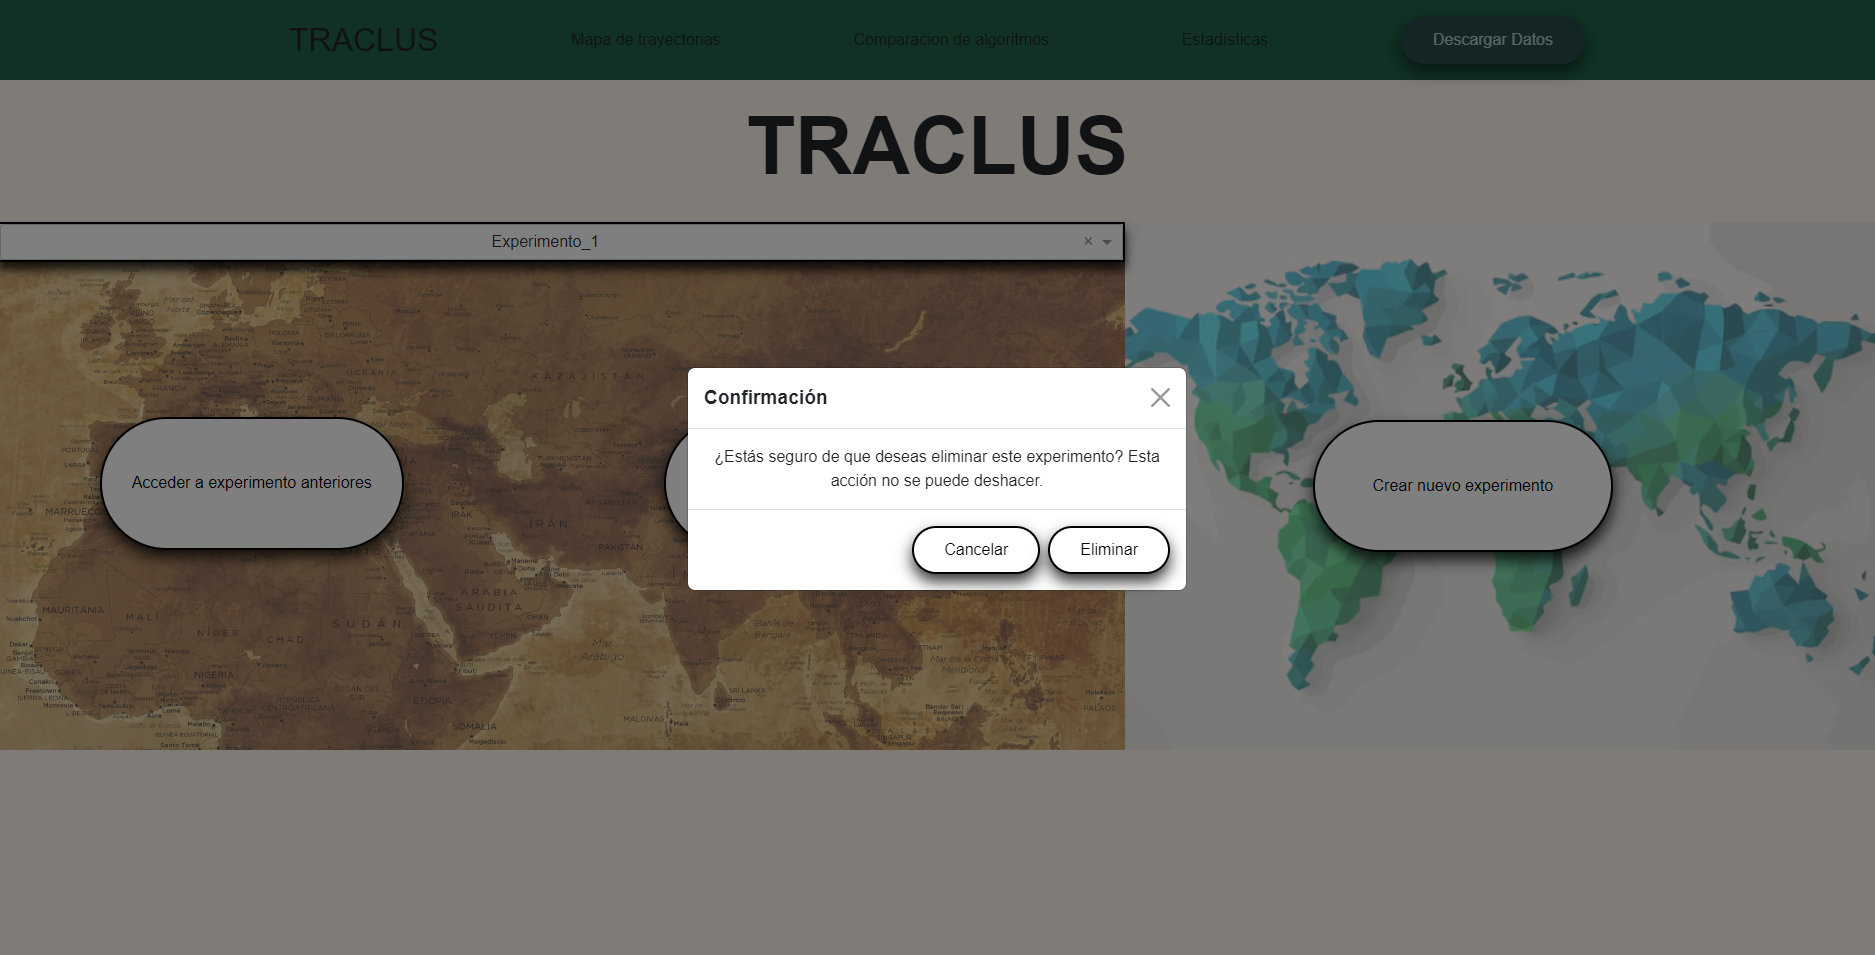
\includegraphics[width=0.9\textwidth]{img/webpage/Delete.png}
    \caption{Modal de confirmación para borrar experimento}
\end{figure}

\subsection{Modales informativos}

Adicionalmente, la aplicación utiliza diversos modales para notificar al usuario sobre situaciones específicas relacionadas con la gestión de experimentos, como la falta de datos o parámetros necesarios.

\begin{figure}[H]
    \centering
    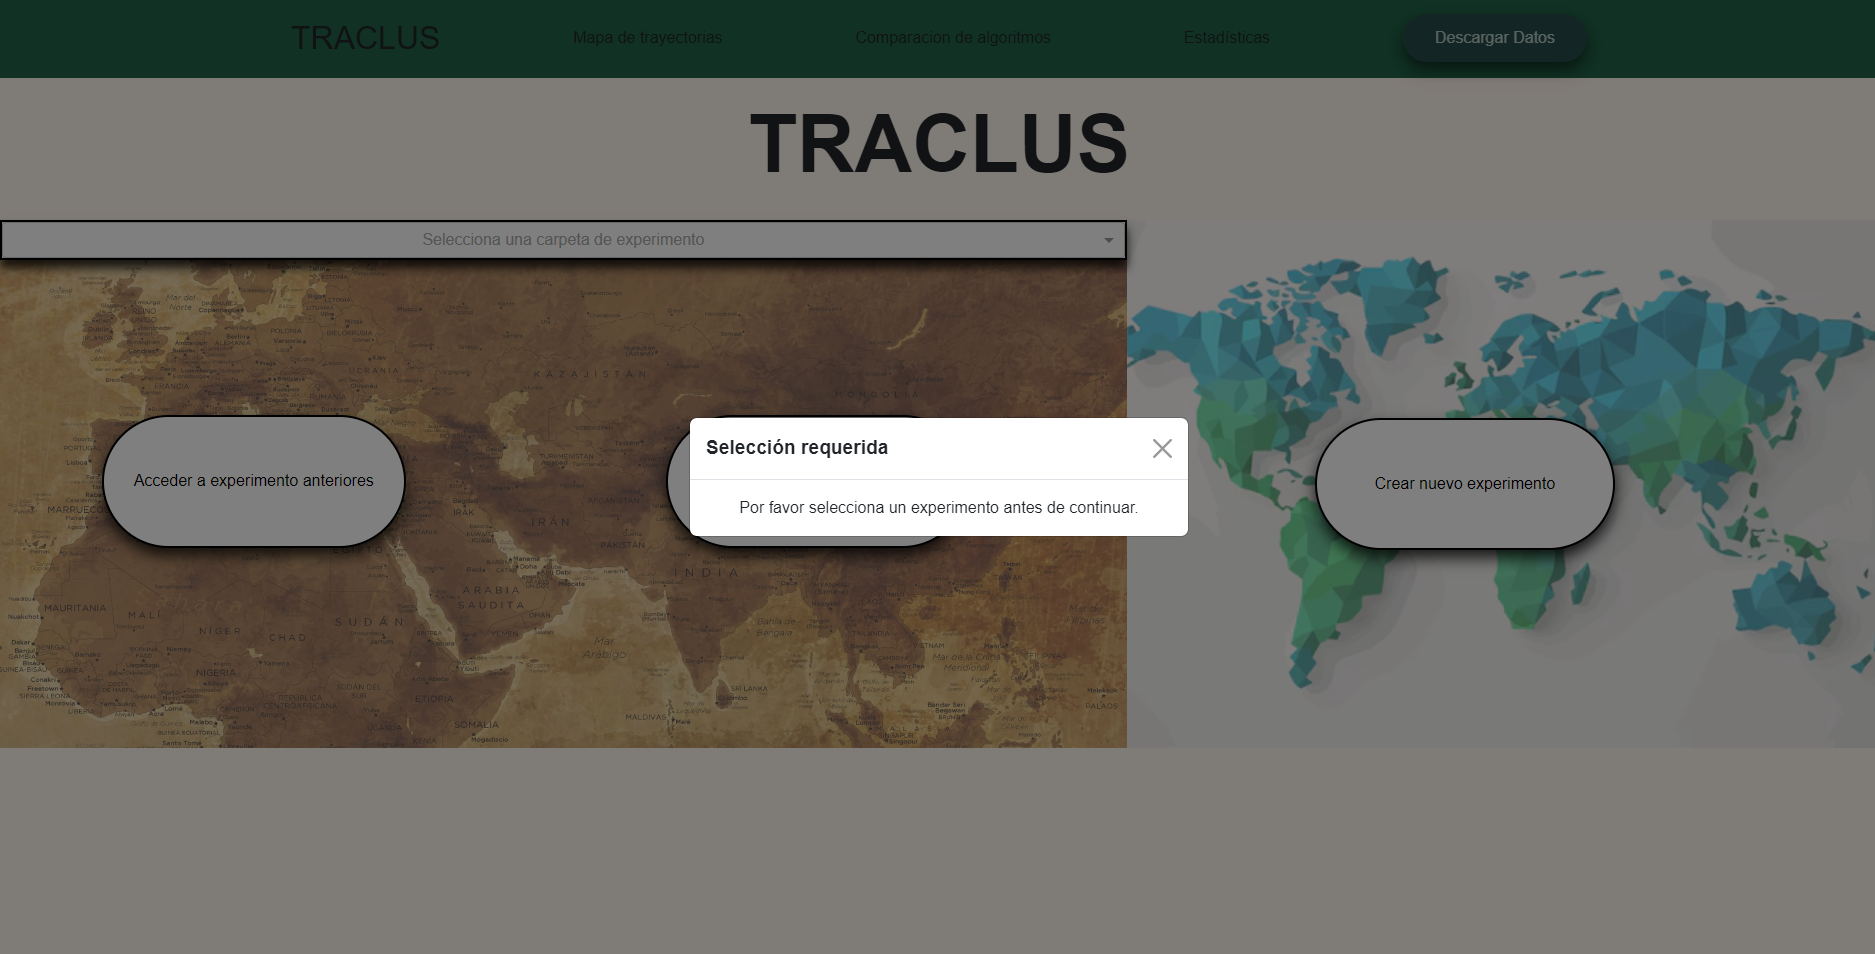
\includegraphics[width=0.9\textwidth]{img/webpage/Modal_1.png}
    \caption{Modal que informa al usuario sobre la ausencia de un experimento seleccionado.}
\end{figure}

\begin{figure}[H]
    \centering
    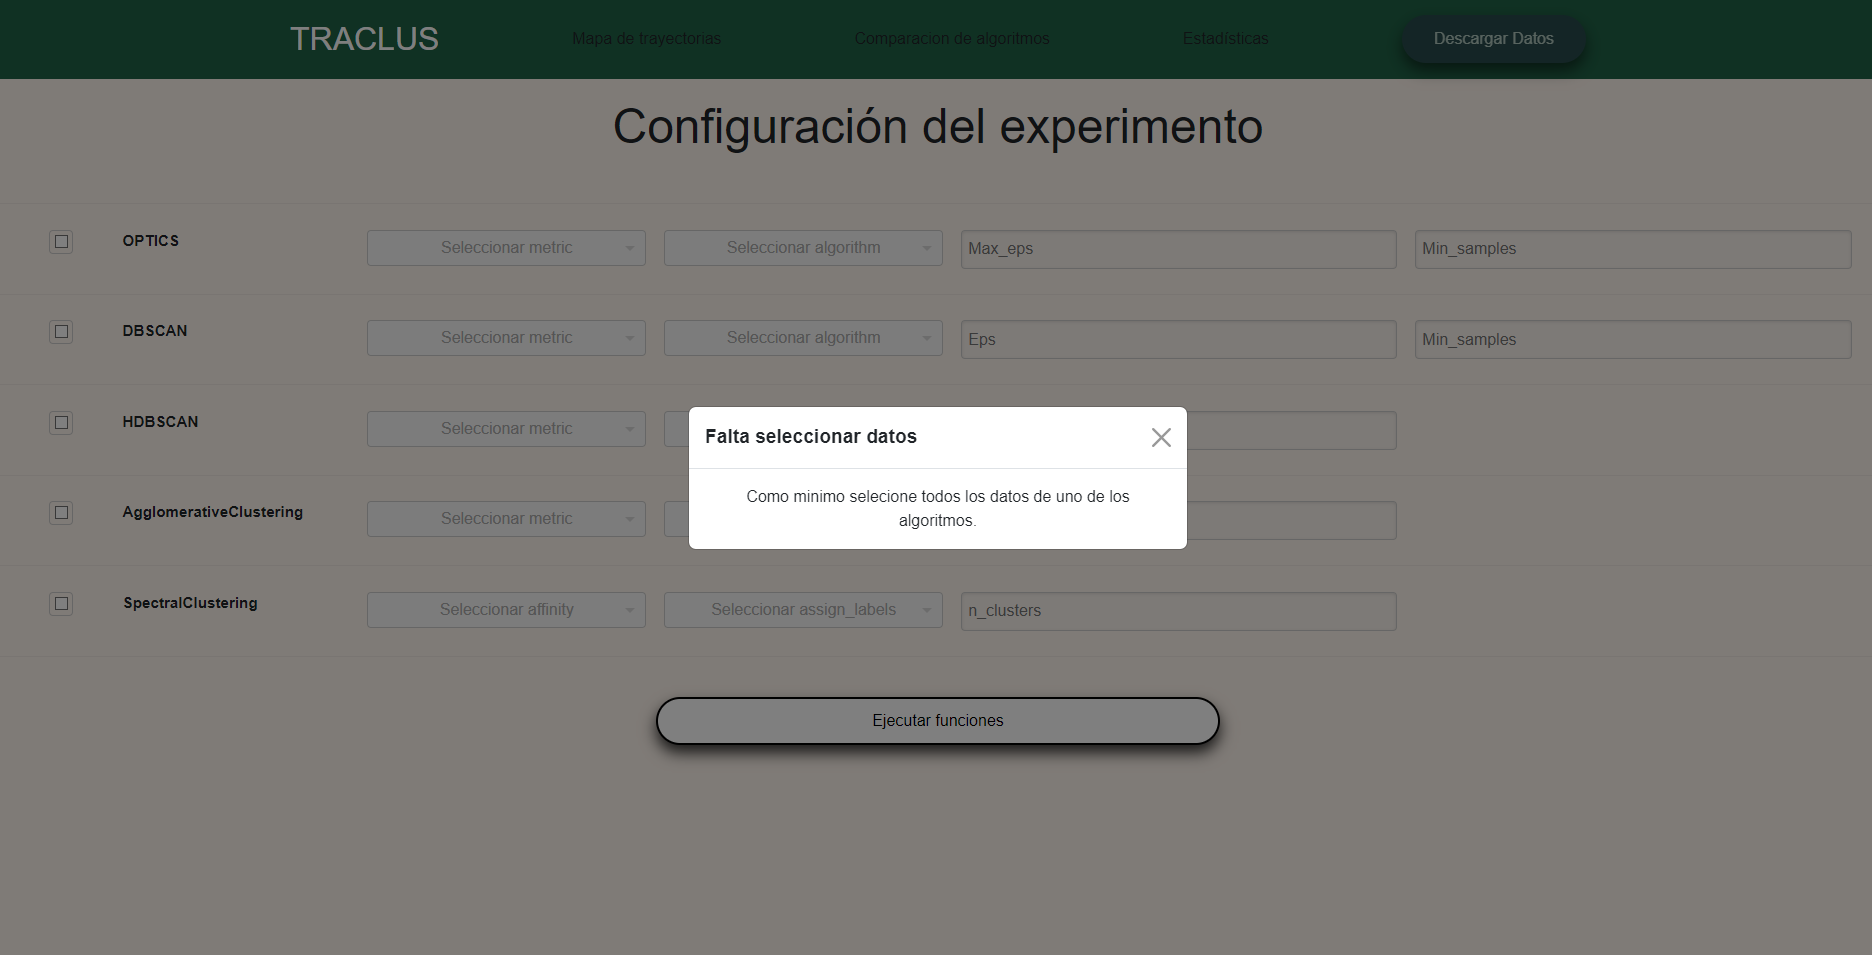
\includegraphics[width=0.9\textwidth]{img/webpage/Modal_2.png}
    \caption{Modal que alerta sobre la falta de parámetros requeridos.}
\end{figure}


